Betrachten Sie folgendes Petrinetz:



\begin{centering}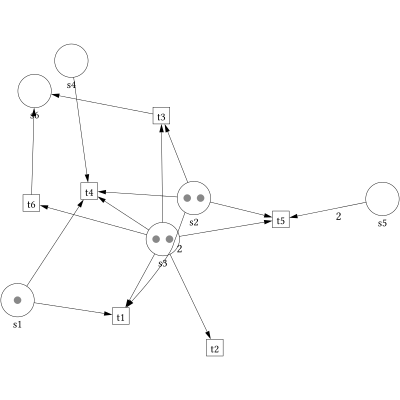
\includegraphics[min width=0.4\textwidth=0.6\textwidth,min height=0.4\textwidth=0.6\textwidth,keepaspectratio,max width=0.9\textwidth,max height=0.9\textwidth]{66/conflictpetri47bb63cb0231e8a3361e3b58708c9231bb7f67b73402a4e9a996482a4959978811011.pdf}\end{centering}

Welches Paar von Transitionen steht in Konflikt, und wegen welcher konfliktverursachenden Stelle(n), unter der Startmarkierung?

Geben Sie Ihre Antwort durch Angabe eines Paars von in Konflikt stehenden Transitionen und einer Liste aller Stellen, die den Konflikt verursachen. Die Angabe von \begin{verbatim}((t0,t1),[s0,s1])\end{verbatim} als Antwort würde bedeuten, dass Transitionen t0 und t1 unter der Startmarkierung in Konflikt stehen
und dass die Stellen s0 und s1 all jene gemeinsamen Stellen in den Vorbedingungen sind,
die jeweils einzeln nicht ausreichend Marken zum gleichzeitigen Feuern der Transitionen t0 und t1 haben. Die Reihenfolge der Transitionen innerhalb des zuerst angegebenen Paars spielt hierbei keine Rolle.
Die Reihenfolge von Stellen innerhalb der Auflistung der den Konflikt verursachenden Stellen spielt ebenso keine Rolle.

Bitte beachten Sie: Beim Bewegen über oder Klicken auf Kanten / Knoten bzw. ihre Beschriftungen werden die jeweils zusammengehörenden Komponenten hervorgehoben.

